%****************************************************************************************************
% Modelo criado por Vinícius Barros Rodrigues (viniciusbrbio@gmail.com)
% versão 0.6
% Setembro 2016
% Disponível em: https://github.com/ViniciusBRodrigues/TeseUFVLatex
%****************************************************************************************************
% Pacotes
%****************************************************************************************************
\documentclass[12pt]{report}
\usepackage[utf8]{inputenc}
\usepackage[brazilian,brazil]{babel}
\usepackage[a4paper,left=4cm,right=3cm,bottom=2.5cm,top=2.8cm]{geometry}
\usepackage{fancyhdr,setspace,float,graphicx,lscape,array,longtable,colortbl,amsmath,amssymb,booktabs,multirow,hyperref,pdfpages,tocloft,titlesec,natbib,lipsum}
\renewcommand\cftloftitlefont{\Large\bfseries\hfill}
\renewcommand\cftlottitlefont{\Large\bfseries\hfill}
\renewcommand\cfttoctitlefont{\Large\bfseries\hfill}
\titleformat{\chapter}[display]
{\vspace*{-0.7cm}\bfseries\Huge}
{\filleft{\chaptertitlename}\Huge~\thechapter}
{1ex}
{\titlerule
\vspace{2ex}%
\filright}
[]

%****************************************************************************************************
% Fontes Palladio
\usepackage[sc]{mathpazo}
\linespread{1.05}
\usepackage[T1]{fontenc}
%****************************************************************************************************
% Coloque suas imagens e gráficos na pasta images
\graphicspath{{imagens/}}
%****************************************************************************************************

\begin{document}

%****************************************************************************************************
% Edite cada um dos seguintes arquivos na pasta "preamble"
%****************************************************************************************************


   \thispagestyle{empty}
   \setcounter{page}{0}
\begin{spacing}{1}
	\begin{center}
		\vspace*{-0.5cm}
		{\MakeUppercase{Seu Nome Completo} \\ }
		
		% Título
		
		\vspace*{8cm}
		{\MakeUppercase{\textbf{Título da sua tese}} \\ }
	\end{center}
	%
	\vspace*{4cm}
	\singlespacing
	\begin{flushright}
		\begin{minipage}{7.5cm}
			{Tese apresentada à Universidade Federal de Viçosa, como parte
				das exigências do Programa de Pós-Graduação em PROGRAMA, para
				obtenção do título de \textit{NOME DO TÍTULO}.}
		\end{minipage}
	\end{flushright}
	\vfill
	
	\begin{center}
	VIÇOSA
	
	MINAS GERAIS - BRASIL
	
	Julho - 2016
	
	
	\end{center}
	
\end{spacing}


\newpage
 \thispagestyle{empty}
% \pagenumbering{roman}
% \doublespacing
 \setcounter{page}{1}
\begin{spacing}{1}
\begin{center}
% \vspace*{-0.5cm}
{\MakeUppercase{Seu Nome Completo} \\ }

\vspace*{4.2cm}
{\MakeUppercase{\textbf{Título da sua tese}} \\ }
\end{center}

\vspace*{2.6cm}
\singlespacing
\begin{flushright}
\begin{minipage}{7.5cm}
{Tese apresentada à Universidade Federal de Viçosa, como parte
  das exigências do Programa de Pós-Graduação em PROGRAMA, para
  obtenção do título de \textit{NOME DO TÍTULO}.}
\end{minipage}
\end{flushright}
\vspace*{1.3cm}
%
% % Data de aprovação. Mês por extenso.
%
APROVADA: DIA de MÊS de ANO.
\vfill
%
% % Componentes da banca
%
\begin{minipage}{0.45\linewidth}
\centering
\vspace{0.5cm}
\rule{\linewidth}{0.1mm}\\
{Membro da banca 1}%%%%%%%%%%%%%%%%%%% Membro 1
\end{minipage}
\hfill
\begin{minipage}{0.45\linewidth}
\centering
\vspace*{0.5cm}
\rule{\linewidth}{0.1mm}
{Membro da banca 2}%%%%%%%%%%%%%%%%%%% Membro 2
\end{minipage}
\vfill
\begin{minipage}{0.45\linewidth}
\centering
\rule{\linewidth}{0.1mm}
{Membro da banca 3}%%%%%%%%%%%%%%%%%%% Membro 3
\end{minipage}
\hfill
\begin{minipage}{0.45\linewidth}
\centering
\rule{\linewidth}{0.1mm}
{Membro da banca 4}%%%%%%%%%%%%%%%%%%% Membro 3
\end{minipage}

\vfill
\begin{center}
\begin{minipage}{7.5cm}
{\begin{center}
\rule{\linewidth}{0.1mm} \\
{Membro da banca 5}\\%%%%%%%%%%%%%%%%%%% Orientador
(Orientador)
\end{center}}
\end{minipage}
\end{center}
\end{spacing}


\clearpage
\onehalfspacing
\pagenumbering{roman}
\setcounter{page}{2}
\pagestyle{fancy}
\fancyhead{}
\fancyhead[RO,LE]{\thepage}
\fancyfoot{}
\fancyfoot[LE,RO]{}
\fancyfoot[LO,CE]{}
\fancyfoot[CO,RE]{}
\vspace*{0.7cm}
\section*{\hfill Dedicatória}
\vspace*{\fill}
%%%%%%%%%%%%%%%%%%%%%%%%%%%%%%%%%%%%%%%%%%%%%%%%%%%%%%%%%%%%%%%%%%%%%%%%%%%%%%%%%%%%%%%%%%%%%%%%%%%%%%%%%%%%%%%%%%%%%%%%%%%%%%%%%%%%%%%%%%%%%%%%
\begin{flushright}
Sua Dedicatória aqui.
\end{flushright}
%%%%%%%%%%%%%%%%%%%%%%%%%%%%%%%%%%%%%%%%%%%%%%%%%%%%%%%%%%%%%%%%%%%%%%%%%%%%%%%%%%%%%%%%%%%%%%%%%%%%%%%%%%%%%%%%%%%%%%%%%%%%%%%%%%%%%%%%%%%%%%%%

\clearpage
\pagestyle{fancy}
\fancyhead{}
\fancyhead[RO,LE]{\thepage}
\fancyfoot{}
\fancyfoot[LE,RO]{}
\fancyfoot[LO,CE]{}
\fancyfoot[CO,RE]{}
\vspace*{0.7cm}
\section*{\hfill Epígrafe}
\vspace*{\fill}
%%%%%%%%%%%%%%%%%%%%%%%%%%%%%%%%%%%%%%%%%%%%%%%%%%%%%%%%%%%%%%%%%%%%%%%%%%%%%%%%%%%%%%%%%%%%%%%%%%%%%%%%%%%%%%%%%%%%%%%%%%%%%%%%%%%%%%%%%%%%%%%%
\begin{flushright}
Sua Epígrafe aqui.
\end{flushright}
%%%%%%%%%%%%%%%%%%%%%%%%%%%%%%%%%%%%%%%%%%%%%%%%%%%%%%%%%%%%%%%%%%%%%%%%%%%%%%%%%%%%%%%%%%%%%%%%%%%%%%%%%%%%%%%%%%%%%%%%%%%%%%%%%%%%%%%%%%%%%%%%



\clearpage
\pagestyle{fancy}
\fancyhead{}
\fancyhead[RO,LE]{\thepage}
\fancyfoot{}
\fancyfoot[LE,RO]{}
\fancyfoot[LO,CE]{}
\fancyfoot[CO,RE]{}
\vspace*{0.7cm}
\section*{\hfill Agradecimentos}
\vspace{0.5cm}
%%%%%%%%%%%%%%%%%%%%%%%%%%%%%%%%%%%%%%%%%%%%%%%%%%%%%%%%%%%%%%%%%%%%%%%%%%%%%%%%%%%%%%%%%%%%%%%%%%%%%%%%%%%%%%%%%%%%%%%%%%%%%%%%%%%%%%%%%%%%%%%%
% Seu texto aqui











%%%%%%%%%%%%%%%%%%%%%%%%%%%%%%%%%%%%%%%%%%%%%%%%%%%%%%%%%%%%%%%%%%%%%%%%%%%%%%%%%%%%%%%%%%%%%%%%%%%%%%%%%%%%%%%%%%%%%%%%%%%%%%%%%%%%%%%%%%%%%%%%
\newpage

%****************************************************************************************************
% Sumário
\normalsize
\tableofcontents
\newpage
\listoffigures
\addcontentsline{toc}{section}{\listfigurename}
\newpage
\listoftables
\addcontentsline{toc}{section}{\listtablename}
%****************************************************************************************************

\clearpage
\vspace*{0.7cm}
\section*{\hfill Resumo}
\vspace{1cm}
%%%%%%%%%%%%%%%%%%%%%%%%%%%%%%%%%%%%%%%%%%%%%%%%%%%%%%%%%%%%%%%%%%%%%%%%%%%%%%%%%%%%%%%%%%%%%%%%%%%%%%%%%%%%%%%%%%%%%%%%%%%%%%%%%%%%%%%%%%%%%%%%
% Seu resumo aqui

\lipsum[2-2]




%%%%%%%%%%%%%%%%%%%%%%%%%%%%%%%%%%%%%%%%%%%%%%%%%%%%%%%%%%%%%%%%%%%%%%%%%%%%%%%%%%%%%%%%%%%%%%%%%%%%%%%%%%%%%%%%%%%%%%%%%%%%%%%%%%%%%%%%%%%%%%%%

%****************************************************************************************************
% Edite cada um dos seguintes arquivos na pasta "capitulos"
% Apenas comente ou descomente de acordo com o que precisar
%****************************************************************************************************

\clearpage
\pagenumbering{arabic}
\setcounter{page}{1}
\pagestyle{fancy}
\fancyhead{}
\fancyhead[RO,LE]{Título da tese (opcional)} %%%% preencher (opcional)
\fancyfoot{}
\fancyfoot[LE,RO]{\thepage}
\fancyfoot[LO,CE]{Capítulo \thechapter}
\fancyfoot[CO,RE]{Autor (opcional)} %%%% preencher com nome (opcional)
%%%%%%%%%%%%%%%%% COLE SEU TEXTO AQUI: %%%%%%%%%%%%%%%%%%%%%%%
\chapter{\sc Um título}
\lipsum[2-2] \citep{lamport1986latex} 
\begin{figure}[h]
\centering
\caption{Minha figura}
 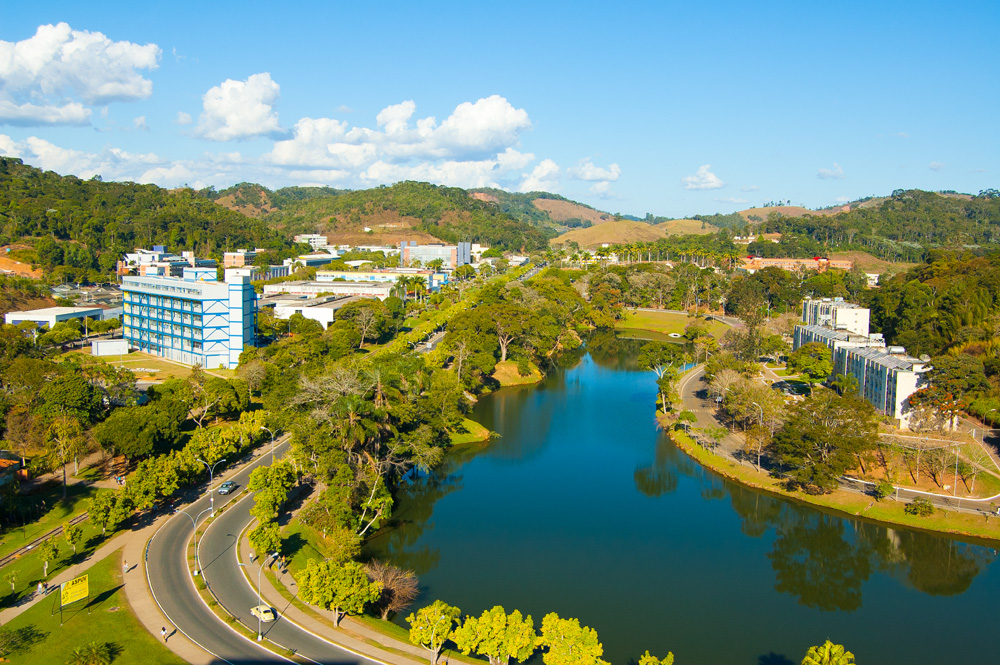
\includegraphics[scale=0.2]{ufv.jpg}
\end{figure}
\section{Seção nova}
\lipsum[2-3]
%%%% APAGAR O EXEMPLO ACIMA








%
\chapter{\sc Título do capítulo}
\lipsum[2-4] \cite{kopka2004guide}\lipsum[1]
\begin{table}[]
\centering
\caption{Minha tabela}
\label{my-label}
\begin{tabular}{lll}
1 & a & s \\ \hline
1 & a & x \\
2 & z & s
\end{tabular}
\end{table}

%%%% APAGAR O EXEMPLOS ACIMA
%
% se necessário, acrescente outros capítulos;
% \input{capitulos/cap03}

%****************************************************************************************************
% Referências
\clearpage
\phantomsection
\addcontentsline{toc}{chapter}{Referências Bibliográficas}
\bibliographystyle{apalike}
\bibliography{referencias.bib} %%% nome do seu arquivo .bib

%****************************************************************************************************
% Análises estatísticas em pdf
% Descomente e coloque o nome do seu arquivo
%\includepdf[pages=-]{myfile.pdf}
%****************************************************************************************************
  
\end{document}
